\documentclass[unicode,14pt]{beamer}
\usepackage{mypresentation}
%\usepackage{yafootnote-beamer}
\protected\def\pdfliteral{\pdfextension literal}

\def\bftncm{\texttt{\bfseries\textbackslash{}footnote}}
\def\nftncm{\texttt{\textbackslash{}footnote}}

\title{\bftncm{}再考}
\author{\sffamily 鹿野 桂一郎\\
\bfseries ラムダノート株式会社\\
\small\bfseries \email{k16.shikano@lambdanote.com} \\ 
\twitter{golden\_lucky} 
}
\date{\sffamily\footnotesize 2023年11月11日\\ 於\, TeXConf 2023}

\begin{document}

\frame{\titlepage}

\setbeamertemplate{background canvas}[vertical shading][bottom=white,top=kachi!15]
\setbeamercolor{frametitle}{bg=kachi, fg=white}
\setbeamercolor{structure}{fg=kachi}

\begin{frame}[t]{\inhibitglue \bftncm{}の挙動が気に食わない}
  \sffamily
  \begin{itemize}
    \item ボックスの中で使ってもページ下部に出てほしい
    \item ボックスが改ページしてもページ下部に出てほしい
    \item 脚注にも脚注を付けたい
  \end{itemize}
  \vfill
\end{frame}

\begin{frame}[t]{自分で作ろう!でもどうやって?}
  \sffamily
  \begin{itemize}
    \item \TeX{}の脚注は「インサート」という謎機能
    \item 直感的に思いつく素直な実装方法は、むしろこんな感じではないだろうか?
  \end{itemize}
  
  ↓
  
  \begin{enumerate}
    \item 脚注の内容のみをブロック要素として組版
    \item アンカーのあるインライン要素に紐づける形で、そのブロック要素をいったん保持
    \item ページ分割時に、もしアンカーがあったら、紐づけられているブロック要素の高さを考慮する
    \item そのページの下部に、そのブロック要素を配置する
  \end{enumerate}
\end{frame}

\begin{frame}[t]{\TeX{}だけでは(たぶん)無理}
  \sffamily
  \begin{itemize}
\item 少なくとも、インサートを使う方法では無理そう(後述)
\item 行分割やページ分割に割り込んでレジスタやトークンリストの操作ができるようになれば、あるいは…
\item そういえば最近の\LaTeX{}カーネルには「フック」とかいう機能が導入されていたような
  \end{itemize}
\end{frame}

\begin{frame}[t]{\LaTeX{}のフックでも(たぶん)無理}
  \sffamily
  \begin{itemize}
\item \TeX{}エンジンレベルの処理には割り込めない
\item \LaTeX{}ラボ\footnote{\url{https://ctan.org/tex-archive/macros/latex/required/latex-lab}}には\nftncm{}に関するフックもあるが、これらの対象は事実上\texttt{\textbackslash{}@footnotemark}と\texttt{\textbackslash{}@footnotetext}なので、結局はインサートとして読まれてしまってダメ(後述)
  \end{itemize}
\end{frame}


\begin{frame}[t]{そこでLua\TeX}
  \sffamily
  \begin{itemize}
\item Luaのオブジェクトとして構文木(っぽいもの)が作られる\\
    \begin{itemize} 
\item node listと呼ばれている\footnote{\url{https://ctan.org/pkg/nodetree}}
\item node listに対する操作として、行分割処理の前後などで発動するフックが書ける\footnote{\url{https://wiki.luatex.org/index.php/Callbacks}}
    \end{itemize} 
\item \texttt{\textbackslash{}attribute}という新しいプリミティブが使える\\
    \begin{itemize} 
\item LuaのオブジェクトとTeXのコードとの間で、メタ情報をやり取りできる\footnote{\url{https://wiki.luatex.org/index.php/Attributes}}
    \end{itemize} 
  \end{itemize} 
\end{frame}

\begin{frame}[t]{実装の方針}
  \begin{itemize}
\item \nftncm{}を見たら以下をする。
  \end{itemize}

\vskip\baselineskip

  \begin{enumerate}
\item \nftncm{}の中身をとりあえず組む
\item その行の直下に配置
\item 脚注マークと紐づける
\item 組んだ要素の高さと深さをつぶす
\item その要素をページ下部へ
  \end{enumerate} 
\end{frame}

\begin{frame}[t]{実装の方針}
  \begin{itemize}
\item \nftncm{}を見たら以下をする。
  \end{itemize}

\vskip\baselineskip

  \begin{enumerate}
\item \nftncm{}の中身をとりあえず組む
\item その行の直下に配置 {\color{red} ← \texttt{post\_linebreak\_filter}}
\item 脚注マークと紐づける {\color{red} ← \texttt{\textbackslash{}attribute}}
\item 組んだ要素の高さと深さをつぶす {\color{red} ← \texttt{vpack\_filter}}
\item その要素をページ下部へ {\color{red} ← \texttt{pre\_output\_filter}}
  \end{enumerate} 
\end{frame}

\begin{frame}[fragile]{\texttt{post\_linebreak\_filter}}
\scriptsize
\begin{Shaded}
\begin{Highlighting}[]
\VariableTok{push\_footnotes\_below\_lines} \OperatorTok{=} \KeywordTok{function} \OperatorTok{(}\VariableTok{head}\OperatorTok{,} \VariableTok{group}\OperatorTok{)}
  \ControlFlowTok{for} \VariableTok{item} \KeywordTok{in} \VariableTok{node}\OperatorTok{.}\NormalTok{traverse\_id}\OperatorTok{(}\VariableTok{node}\OperatorTok{.}\NormalTok{id}\OperatorTok{(}\StringTok{"whatsit"}\OperatorTok{),} \VariableTok{head}\OperatorTok{)} \ControlFlowTok{do}
    \KeywordTok{local} \VariableTok{is\_footnote} \OperatorTok{=} \VariableTok{node}\OperatorTok{.}\NormalTok{has\_attribute}\OperatorTok{(}\VariableTok{item}\OperatorTok{,} \DecValTok{100}\OperatorTok{)}
    \ControlFlowTok{if} \VariableTok{is\_footnote} \KeywordTok{and} \VariableTok{is\_footnote} \OperatorTok{\textgreater{}} \DecValTok{0} \ControlFlowTok{then}
      \KeywordTok{local} \VariableTok{footnote} \OperatorTok{=} \VariableTok{node}\OperatorTok{.}\NormalTok{copy}\OperatorTok{(}\VariableTok{tex}\OperatorTok{.}\VariableTok{box}\OperatorTok{[}\VariableTok{is\_footnote}\OperatorTok{])}
      \VariableTok{head}\OperatorTok{,} \VariableTok{new} \OperatorTok{=} \VariableTok{node}\OperatorTok{.}\NormalTok{insert\_after}\OperatorTok{(}\VariableTok{head}\OperatorTok{,} \VariableTok{item}\OperatorTok{,} \VariableTok{footnote}\OperatorTok{)}
      \VariableTok{item} \OperatorTok{=} \VariableTok{item}\OperatorTok{.}\VariableTok{next}
    \ControlFlowTok{end}
  \ControlFlowTok{end}
  \ControlFlowTok{return} \VariableTok{head}
\KeywordTok{end}

\VariableTok{luatexbase}\OperatorTok{.}\VariableTok{add\_to\_callback}
  \OperatorTok{(}\StringTok{"post\_linebreak\_filter"}\OperatorTok{,}\VariableTok{push\_footnotes\_below\_lines}\OperatorTok{,}\StringTok{"pushftn"}\OperatorTok{)}
\end{Highlighting}
\end{Shaded}
\end{frame}

\begin{frame}[fragile]{Whatsitに\texttt{\textbackslash{}attribute}\footnote{この手法についてはTUGboat, Volume 31 (2010), No. 3のPaul Isambertによる記事\url{https://tug.org/tugboat/tb31-3/tb99isambert.pdf}が参考になる。}を付与}
\scriptsize
\begin{Shaded}
\begin{Highlighting}[]
\FunctionTok{\textbackslash{}def\textbackslash{}yafootnote}\NormalTok{\#1\{}\FunctionTok{\textbackslash{}nobreak}\CommentTok{\%}
  \FunctionTok{\textbackslash{}global\textbackslash{}advance\textbackslash{}yafootnotecount}\NormalTok{ 1}
  \FunctionTok{\textbackslash{}global\textbackslash{}expandafter\textbackslash{}newbox}
    \FunctionTok{\textbackslash{}csname}\NormalTok{ yafoot\_}\FunctionTok{\textbackslash{}the\textbackslash{}yafootnotecount\textbackslash{}endcsname}
  \FunctionTok{\textbackslash{}begingroup}
    {\bfseries\FunctionTok{\textbackslash{}attribute}\NormalTok{100=}\FunctionTok{\textbackslash{}expandafter\textbackslash{}the\textbackslash{}csname}}
      {\bfseries\NormalTok{ yafoot\_}\FunctionTok{\textbackslash{}the\textbackslash{}yafootnotecount\textbackslash{}endcsname}}
    \FunctionTok{\textbackslash{}expandafter\textbackslash{}yafootnotemark\textbackslash{}expandafter}\NormalTok{\{}\FunctionTok{\textbackslash{}the\textbackslash{}yafootnotecount}\NormalTok{\}}
    {\bfseries\FunctionTok{\textbackslash{}vadjust}\NormalTok{ \{}\FunctionTok{\textbackslash{}pdfliteral}\NormalTok{\{\}\}}\CommentTok{\%}}
  \FunctionTok{\textbackslash{}endgroup}
  \FunctionTok{\textbackslash{}global\textbackslash{}expandafter\textbackslash{}setbox}
    \FunctionTok{\textbackslash{}csname}\NormalTok{ yafoot\_}\FunctionTok{\textbackslash{}the\textbackslash{}yafootnotecount\textbackslash{}endcsname}
    \FunctionTok{\textbackslash{}vtop}\NormalTok{\{}\FunctionTok{\textbackslash{}yafootnotetext}\NormalTok{\{\#1\}\}\}}
\end{Highlighting}
\end{Shaded}
\end{frame}

\begin{frame}[t]{\texttt{post\_linebreak\_filter}後}
\begin{center}
\colorbox{white}{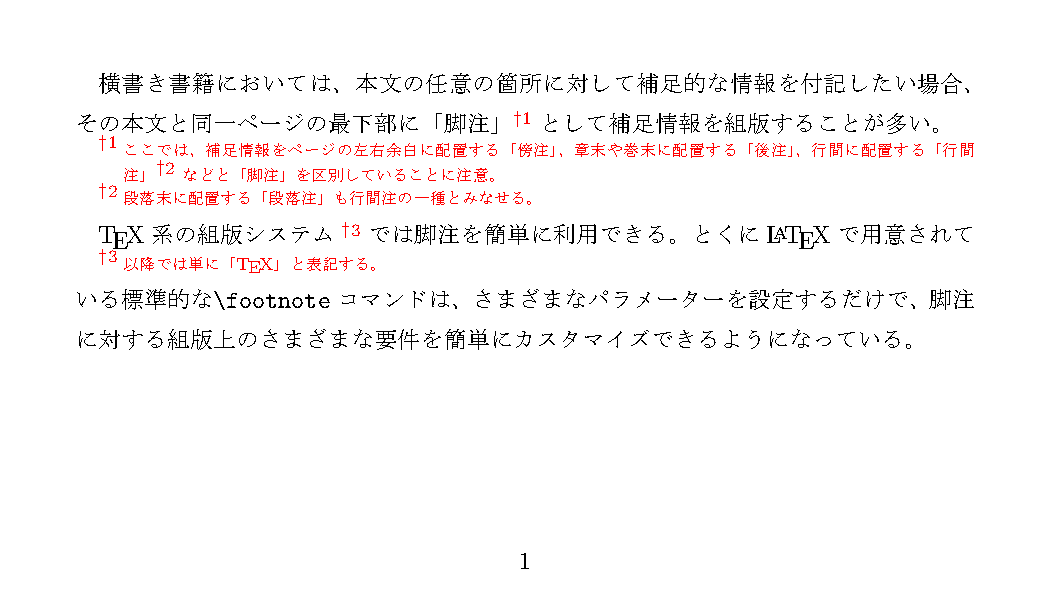
\includegraphics[width=.9\textwidth]{codes/history1.pdf}}
\end{center}
\end{frame}

\begin{frame}[fragile]{\texttt{vpack\_filter}}
\scriptsize
\begin{Shaded}
\begin{Highlighting}[]
\VariableTok{crush\_height\_of\_vlist} \OperatorTok{=} \KeywordTok{function} \OperatorTok{(}\VariableTok{head}\OperatorTok{,} \VariableTok{group}\OperatorTok{,} \VariableTok{size}\OperatorTok{)}
  \ControlFlowTok{for} \VariableTok{list} \KeywordTok{in} \VariableTok{node}\OperatorTok{.}\NormalTok{traverse\_id}\OperatorTok{(}\VariableTok{node}\OperatorTok{.}\NormalTok{id}\OperatorTok{(}\StringTok{"hlist"}\OperatorTok{),} \VariableTok{head}\OperatorTok{)} \ControlFlowTok{do}
    \ControlFlowTok{for} \VariableTok{item} \KeywordTok{in} \VariableTok{node}\OperatorTok{.}\NormalTok{traverse}\OperatorTok{(}\VariableTok{list}\OperatorTok{)} \ControlFlowTok{do}
      \KeywordTok{local} \VariableTok{f} \OperatorTok{=} \VariableTok{node}\OperatorTok{.}\NormalTok{has\_attribute}\OperatorTok{(}\VariableTok{item}\OperatorTok{,} \DecValTok{200}\OperatorTok{)}
      \ControlFlowTok{if} \VariableTok{f} \ControlFlowTok{then}
        \VariableTok{item}\OperatorTok{.}\VariableTok{height} \OperatorTok{=} \DecValTok{0}
        \VariableTok{item}\OperatorTok{.}\VariableTok{depth} \OperatorTok{=} \DecValTok{0}
      \ControlFlowTok{end}
    \ControlFlowTok{end}
  \ControlFlowTok{end}
  \ControlFlowTok{return} \VariableTok{head}
\KeywordTok{end}

\VariableTok{luatexbase}\OperatorTok{.}\VariableTok{add\_to\_callback}
   \OperatorTok{(}\StringTok{"vpack\_filter"}\OperatorTok{,}\VariableTok{crush\_height\_of\_vlist}\OperatorTok{,}\StringTok{"crushvbox"}\OperatorTok{)}
\end{Highlighting}
\end{Shaded}
\end{frame}

\begin{frame}[t]{\texttt{vpack\_filter}後}
\begin{center}
\colorbox{white}{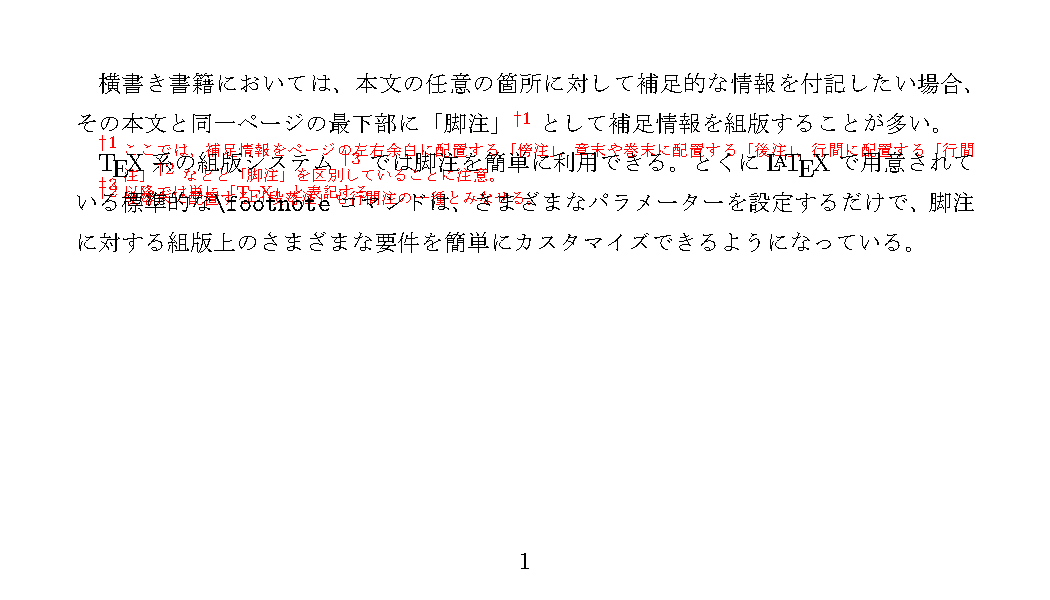
\includegraphics[width=.9\textwidth]{codes/history2.pdf}}
\end{center}
\end{frame}


\begin{frame}[fragile]{\texttt{pre\_output\_filter}}
\tiny%
\begin{Shaded}
\begin{Highlighting}[]
  \VariableTok{move\_footnote\_bottom} \OperatorTok{=} \KeywordTok{function} \OperatorTok{(}\VariableTok{page\_head}\OperatorTok{,} \VariableTok{group}\OperatorTok{,} \VariableTok{s}\OperatorTok{)}
    \KeywordTok{local} \VariableTok{yaftnins} \OperatorTok{=} \VariableTok{node}\OperatorTok{.}\NormalTok{new}\OperatorTok{(}\StringTok{"vlist"}\OperatorTok{)}
    \KeywordTok{local} \VariableTok{n\_head} \OperatorTok{=} \VariableTok{node}\OperatorTok{.}\NormalTok{copy\_list}\OperatorTok{(}\VariableTok{page\_head}\OperatorTok{)}
    \VariableTok{recur} \OperatorTok{=} \KeywordTok{function} \OperatorTok{(}\VariableTok{n}\OperatorTok{)}
      \ControlFlowTok{for} \VariableTok{list} \KeywordTok{in} \VariableTok{node}\OperatorTok{.}\NormalTok{traverse}\OperatorTok{(}\VariableTok{n}\OperatorTok{)} \ControlFlowTok{do}
         \KeywordTok{local} \VariableTok{footnotebox} \OperatorTok{=} \VariableTok{node}\OperatorTok{.}\NormalTok{has\_attribute}\OperatorTok{(}\VariableTok{list}\OperatorTok{,} \DecValTok{200}\OperatorTok{)}
         \ControlFlowTok{if} \VariableTok{footnotebox} \ControlFlowTok{then}
            \VariableTok{footnote} \OperatorTok{=} \VariableTok{node}\OperatorTok{.}\NormalTok{copy}\OperatorTok{(}\VariableTok{tex}\OperatorTok{.}\VariableTok{box}\OperatorTok{[}\VariableTok{footnotebox}\OperatorTok{])}
            \ControlFlowTok{for} \VariableTok{ftnitem} \KeywordTok{in} \VariableTok{node}\OperatorTok{.}\NormalTok{traverse}\OperatorTok{(}\VariableTok{footnote}\OperatorTok{.}\VariableTok{head}\OperatorTok{)} \ControlFlowTok{do}
               \ControlFlowTok{if} \VariableTok{node}\OperatorTok{.}\NormalTok{has\_attribute}\OperatorTok{(}\VariableTok{ftnitem}\OperatorTok{,} \DecValTok{200}\OperatorTok{)} \ControlFlowTok{then}
                  \VariableTok{footnote}\OperatorTok{.}\VariableTok{head} \OperatorTok{=} \VariableTok{node}\OperatorTok{.}\NormalTok{remove}\OperatorTok{(}\VariableTok{footnote}\OperatorTok{.}\VariableTok{head}\OperatorTok{,} \VariableTok{ftnitem}\OperatorTok{)}
               \ControlFlowTok{end}
            \ControlFlowTok{end}
            \ControlFlowTok{if} \VariableTok{yaftnins} \ControlFlowTok{then}
               \VariableTok{yaftnins}\OperatorTok{.}\VariableTok{list}\OperatorTok{,} \VariableTok{new} \OperatorTok{=} \VariableTok{node}\OperatorTok{.}\NormalTok{insert\_after}\OperatorTok{(}\VariableTok{yaftnins}\OperatorTok{.}\VariableTok{list}\OperatorTok{,} \VariableTok{yaftnins}\OperatorTok{.}\VariableTok{tail}\OperatorTok{,} \VariableTok{footnote}\OperatorTok{)}
            \ControlFlowTok{end}
            \VariableTok{n\_head} \OperatorTok{=} \VariableTok{node}\OperatorTok{.}\NormalTok{remove}\OperatorTok{(}\VariableTok{n\_head}\OperatorTok{,} \VariableTok{list}\OperatorTok{)}
            \VariableTok{n\_head} \OperatorTok{=}\NormalTok{ recur}\OperatorTok{(}\VariableTok{list}\OperatorTok{.}\VariableTok{head}\OperatorTok{)}
         \ControlFlowTok{elseif} \VariableTok{list}\OperatorTok{.}\VariableTok{head} \ControlFlowTok{then}
            \VariableTok{n\_head} \OperatorTok{=}\NormalTok{ recur}\OperatorTok{(}\VariableTok{list}\OperatorTok{.}\VariableTok{head}\OperatorTok{)}
         \ControlFlowTok{end}
      \ControlFlowTok{end}
      \ControlFlowTok{return} \VariableTok{n\_head}
   \KeywordTok{end}
   \VariableTok{page\_head} \OperatorTok{=}\NormalTok{ recur}\OperatorTok{(}\VariableTok{n\_head}\OperatorTok{)}
   \ControlFlowTok{if} \VariableTok{yaftnins}\OperatorTok{.}\VariableTok{list} \ControlFlowTok{then}
      \VariableTok{tex}\OperatorTok{.}\VariableTok{box}\OperatorTok{.}\VariableTok{footins} \OperatorTok{=} \VariableTok{node}\OperatorTok{.}\NormalTok{copy}\OperatorTok{(}\VariableTok{node}\OperatorTok{.}\NormalTok{vpack}\OperatorTok{(}\VariableTok{yaftnins}\OperatorTok{.}\VariableTok{list}\OperatorTok{))}
   \ControlFlowTok{end}
   \ControlFlowTok{return} \VariableTok{page\_head}
  \KeywordTok{end}
\end{Highlighting}
\end{Shaded}
\end{frame}

\begin{frame}[t]{\texttt{pre\_output\_filter}後}
\begin{center}
\colorbox{white}{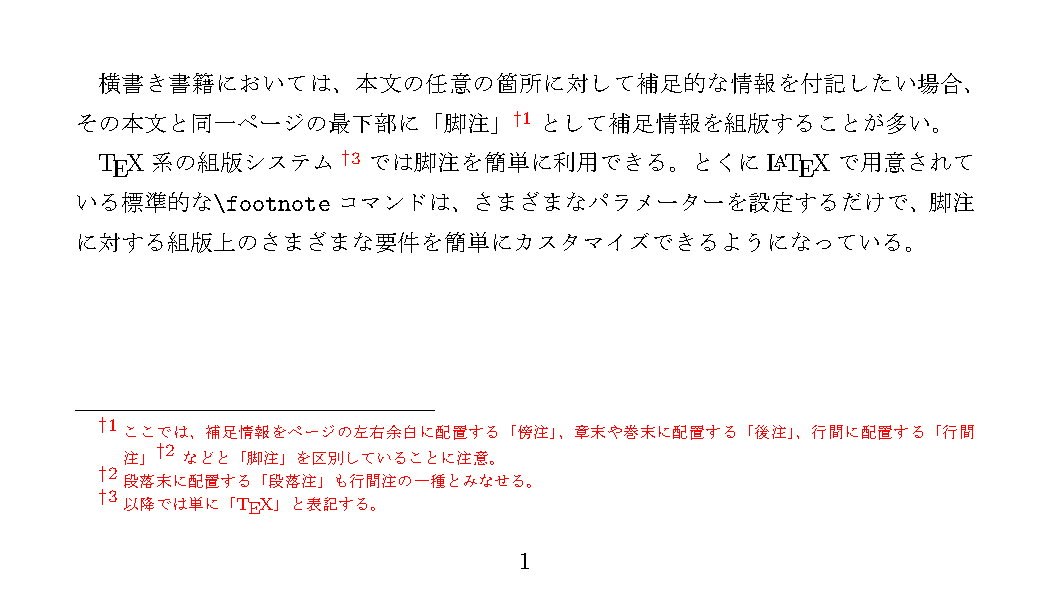
\includegraphics[width=.9\textwidth]{codes/history3.pdf}}
\end{center}
\end{frame}

\begin{frame}[t]{なぜ通常の\bftncm{}ではこれが…}
\begin{itemize}
\item \nftncm{}はインサートで実装されている
\item どのモードであれ、インサートは\textbf{周囲の}垂直リストに入る
\item つまり、もし内部垂直モードなら、\textbf{メイン}垂直リストには入らない
\end{itemize}
\begin{itemize}
\item ページ作成機能が\texttt{\textbackslash{}box255}に移動するのは、\textbf{メイン}垂直リストの要素だけ
\item つまり、内部垂直モードの内側にインサートを置いても、ページ作成機能には届かない!
  \footnote{``The \TeX{}book''には明記されていないようだが``\TeX\ by Topic''などでは説明されている。}
\end{itemize}
\end{frame}

\begin{frame}[t]{原理的にボックス内でも問題ない}
\begin{center}
\colorbox{white}{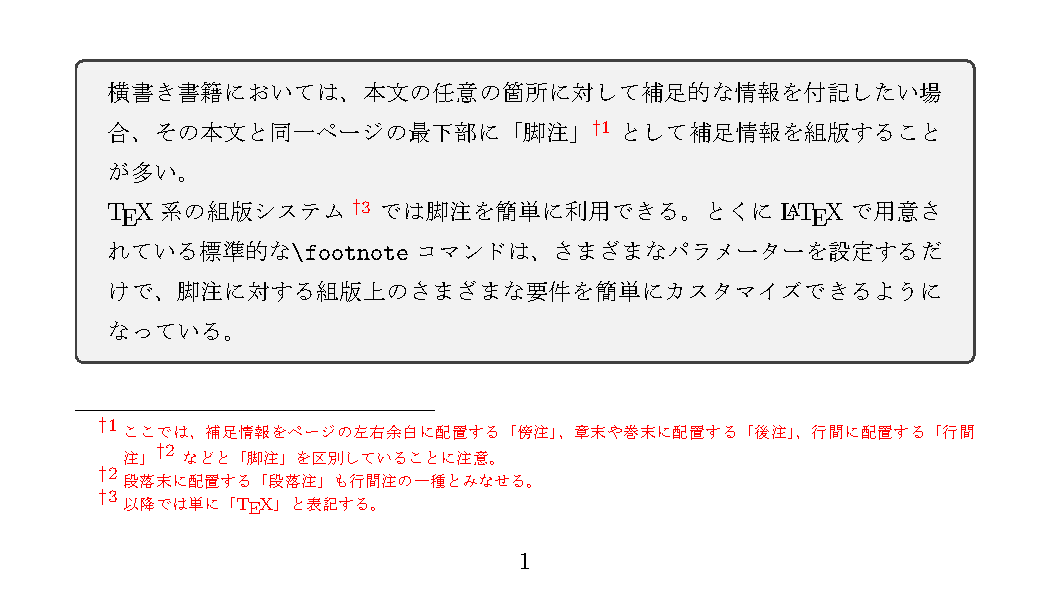
\includegraphics[width=.9\textwidth]{codes/history4.pdf}}
\end{center}
\end{frame}

\begin{frame}[t]{でもページ分割があると…}
\begin{columns}
\begin{column}{0.45\textwidth}
\colorbox{white}{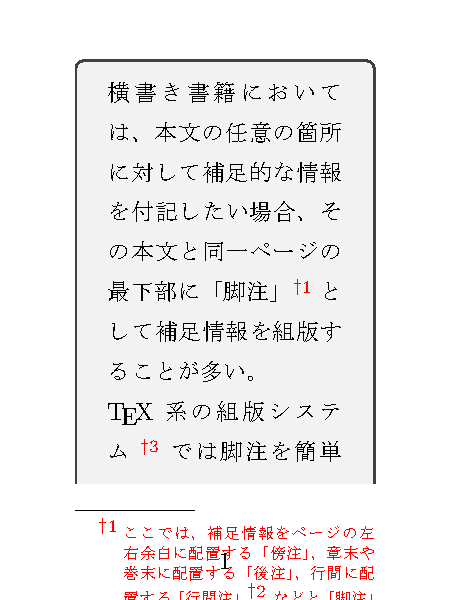
\includegraphics[width=0.9\textwidth, page=1]{codes/history5.pdf}}
\end{column}
\begin{column}{0.45\textwidth}
\colorbox{white}{\includegraphics[width=0.9\textwidth, page=2]{codes/history5.pdf}}
\end{column}
\end{columns}
\end{frame}

\begin{frame}[t]{(tcolorboxの場合の)原因と対処}
\begin{itemize}
\item tcolorboxは\TeX{}のページ作成機能ではなく、\texttt{\textbackslash{}vsplit}を使ってページ分割を手書きしているので\footnote{\url{https://github.com/T-F-S/tcolorbox/blob/18aecbbacc61445c178c3e9a35cadc588b3665bf/tex/latex/tcolorbox/tcbbreakable.code.tex\#L394}}、\texttt{footins}の高さが考慮されない
\item Lua側で「つぶした高さ」を保存しておき、\TeX{}側で用意したディメンジョン(\texttt{\textbackslash{}my@tcb@ftn@height})経由で渡して、
\texttt{\textbackslash{}vsplit}の計算時に考慮するように改造すれば…!
\end{itemize}
\end{frame}

\begin{frame}[fragile]{tcolorboxの分割計算を改造}
\scriptsize%
\begin{Shaded}\begin{Highlighting}[]
{\bfseries\FunctionTok{\textbackslash{}newdimen\textbackslash{}my@tcb@ftn@height}}
{\bfseries\FunctionTok{\textbackslash{}my@tcb@ftn@height\textbackslash{}z@}}

\FunctionTok{\textbackslash{}def\textbackslash{}tcb@vsplit@upper}\NormalTok{\{}\CommentTok{\%}
  {\bfseries\FunctionTok{\textbackslash{}tcbdimto\textbackslash{}tcb@split@dim}\NormalTok{\{}\FunctionTok{\textbackslash{}tcb@split@dim}\NormalTok{{-}}\FunctionTok{\textbackslash{}my@tcb@ftn@height}\NormalTok{\}}}
  {\bfseries\FunctionTok{\textbackslash{}global\textbackslash{}my@tcb@ftn@height\textbackslash{}z@}}
  \FunctionTok{\textbackslash{}setbox\textbackslash{}tcb@upperbox}\NormalTok{=}\FunctionTok{\textbackslash{}vsplit\textbackslash{}tcb@totalupperbox}\NormalTok{ to}\FunctionTok{\textbackslash{}tcb@split@dim}\CommentTok{\%}
  \FunctionTok{\textbackslash{}edef\textbackslash{}tcb@upper@box@badness}\NormalTok{\{}\FunctionTok{\textbackslash{}the\textbackslash{}badness}\NormalTok{\}}\CommentTok{\%}
\NormalTok{  \}}
\end{Highlighting}
\end{Shaded}
\normalsize
\begin{itemize}
\item Lua側ではフック\texttt{buildpage\_filter}を使うことで\texttt{\textbackslash{}my@tcb@ftn@height}を更新
\item 必要な高さを事前計算するため、\texttt{lualatex}を複数回実行
\end{itemize}

\end{frame}


\begin{frame}[t]{顧客が本当に欲しかったもの}

\begin{columns}
\begin{column}{0.3\textwidth}
\colorbox{white}{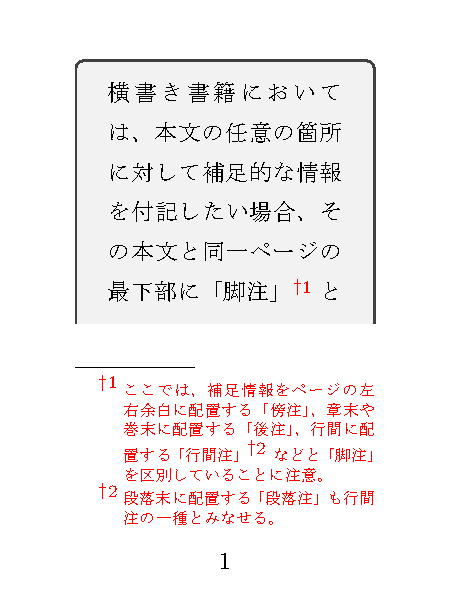
\includegraphics[width=0.9\textwidth, page=1]{codes/history6.pdf}}
\end{column}
\begin{column}{0.3\textwidth}
\colorbox{white}{\includegraphics[width=0.9\textwidth, page=2]{codes/history6.pdf}}
\end{column}
\begin{column}{0.3\textwidth}
\colorbox{white}{\includegraphics[width=0.9\textwidth, page=3]{codes/history6.pdf}}
\end{column}
\end{columns}

\end{frame}

\begin{frame}[t]{課題}
\begin{itemize}
\item ページ分割ボックスの実装方法に応じた個別対応が必要
\item アウトプットルーチンを書き換える必要がある\textbf{場合がある}
\item 浮動要素が同じページに出現する場合の挙動がむずい(最悪、同じ脚注が2回出る)
\item Beamer非対応(ボックス内で独自に脚注を出力させているため)
\item 空いている\texttt{\textbackslash{}attribute}を\TeX{}に生成させたいが、それをLua側から知る方法がわからない
\end{itemize}

\end{frame}

\begin{frame}[t]{でもすぐに使ってみたい!}
\begin{itemize}
\item 第三者につるしで使ってもらうには、もう一息いろいろ整備が必要
\item ラムダノート発行の書籍ではすでに使っています\footnote{株式会社CARTA HOLDINGS 監修、和田卓人 編『事業をエンジニアリングする技術者たち』など。\url{https://www.lambdanote.com/collections/carta}}
\item ソースはGitHubにあるので使ってみることは可能です\\
  \begin{itemize}
\item \url{https://github.com/k16shikano/yafootnote}
  \end{itemize}
\end{itemize}
\end{frame}


\end{document}




\begin{frame}[t]{1. \bftncm{}の中身を行の直下に配置する}
  \sffamily
  \begin{itemize}
\item \nftncm{}の位置にWhatsitノードを挿入し、\texttt{\textbackslash{}attribute100}を設定(\TeX{}側での仕事)
    \begin{itemize}
\item 値は「脚注として組んだものを格納したボックス」の番号
    \end{itemize}
\item 行分割直後に作動するフックで、\texttt{\textbackslash{}attribute100}のWhatsitノードを処理(Lua側での仕事)
    \begin{itemize}
\item 実行する処理は「値に対応する番号のボックスを、新しいノードとして後ろに挿入」
    \end{itemize}
\item 挿入した新しいノードに\texttt{\textbackslash{}attribute200}を設定(Lua側での仕事)
    \begin{itemize}
\item 値は「脚注の中身を脚注として組んだボックス」の番号(\texttt{\textbackslash{}attribute100}と同じ)
    \end{itemize}
  \end{itemize}
\end{frame}

\begin{frame}[t]{2. 行の下に配置したノードをつぶす}
  \sffamily
  \begin{itemize}
\item \TeX{}目線では「\nftncm{}の中身から組まれた垂直リスト」
\item 垂直リスト構築時に作動するフックで、\texttt{\textbackslash{}attribute200}の垂直リストの高さと深さをゼロに
  \end{itemize}
\end{frame}

\begin{frame}[t]{3. つぶしたノードをページ下部に配置}
  \sffamily
  \begin{itemize}
\item \texttt{\textbackslash{}attribute200}が指すボックスの中身を\texttt{\textbackslash{}footins}に直接入れる
\item その際、ボックスの中身も再帰的に処理すれば、入れ子の脚注も\texttt{\textbackslash{}footins}に入る
\item あとは\TeX{}がインサートを考慮して改ページをしてくれる
  \end{itemize}
\end{frame}




